\section{Appendix} \label{sec: Appendix}
The appendix contains code listening and other large information parts that contain partial or complete relevance to the reports topic. 

\subsection{Lesson Learned} \label{subsec: Lesson Learned}
Figure \ref{fig: Vivado_LanguageTemplates} shows a handy tool build into Vivado software package that is called Language Templates and it seems to contain most of the verilog syntax.
\begin{figure}[htbp]
	\centering
	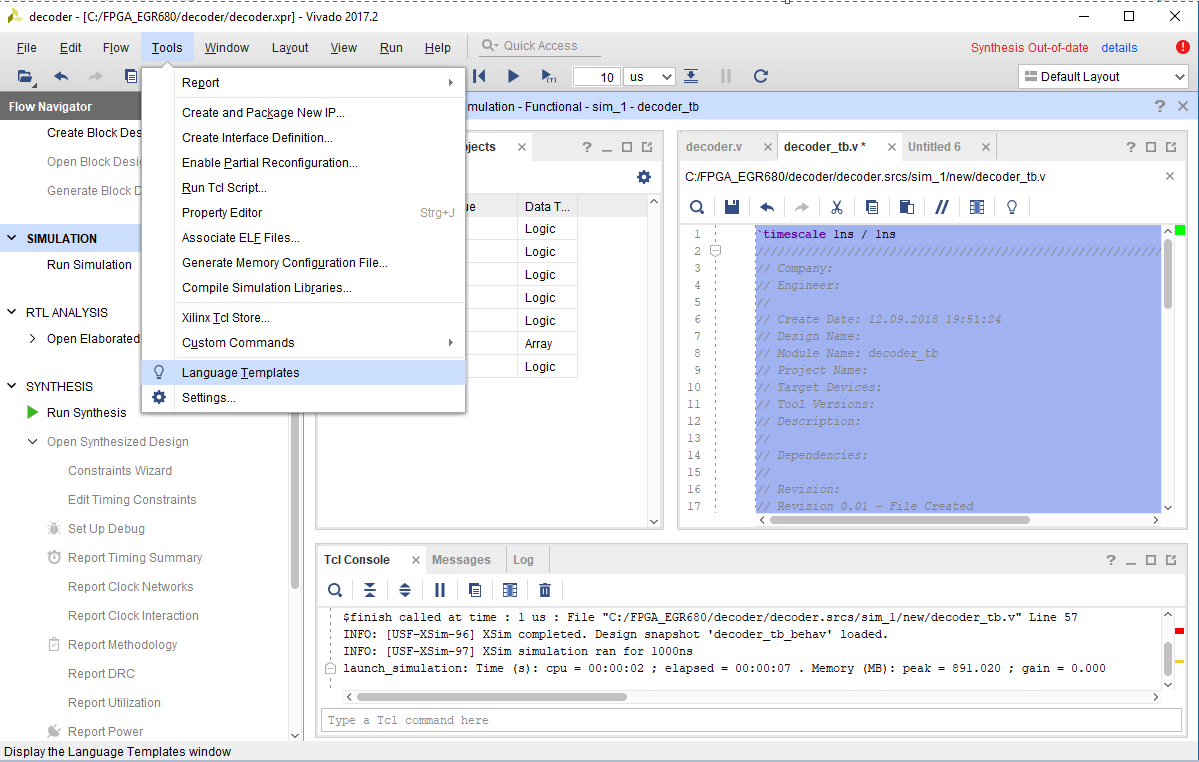
\includegraphics[width=0.6\textwidth]{01_images/Vivado_LanguageTemplates.png}
	\caption{Vivado Language Templates.}
	\label{fig: Vivado_LanguageTemplates}
\end{figure}

\subsection{Part I:Decoder module} \label{subsec: Part I: Decoder module}
\begin{lstlisting}[language=verilog,caption={Testbanche decoder part I.},label=lst: Decoder module]
`timescale 1ns / 1ns
//////////////////////////////////////////////////////////////////////////////////
// Company: 
// Engineer: 
// 
// Create Date: 12.09.2018 19:31:54
// Design Name: 
// Module Name: decoder
// Project Name: 
// Target Devices: 
// Tool Versions: 
// Description: 
// 
// Dependencies: 
// 
// Revision:
// Revision 0.01 - File Created
// Additional Comments:
// 
//////////////////////////////////////////////////////////////////////////////////


module decoder(
input SW0,
input SW1,
input BTN0,
input clk,
input rst,
output [6:0] seg,
output digit
);

reg [6:0] seg;
reg digit;

always @(posedge clk or posedge rst)
begin
if(rst)
begin
seg <= 7'b0000000;
digit <= 1'b1;  // Digit = 1 (7-segment OFF Digit= 0 (7-segment ON)
end
else
begin
// my code or from webpage http://verilogcodes.blogspot.com/2015/10/verilog-code-for-bcd-to-7-segment.html
digit = ~BTN0;
if (BTN0 == 1) begin
case ({SW1, SW0}) //case statement
2'b00 : seg =  7'b0111111; //~7'b0000001;
2'b01 : seg =  7'b0000110;
2'b10 : seg =  7'b1011011;
2'b11 : seg =  7'b1001111;
4 : seg = ~7'b1001100;
5 : seg = ~7'b0100100;
6 : seg = ~7'b0100000;
7 : seg = ~7'b0001111;
8 : seg = ~7'b0000000;
9 : seg = ~7'b0000100;
//switch off 7 segment character when the bcd digit is not a decimal number.
default : seg = 7'b0000000; 
endcase
end
else begin
seg = 7'b0000000; 
end  
end
end
endmodule
\end{lstlisting}

\subsection{Part I: Behavioral simulation of decoder code test bench} \label{subsec: Part I: behavioral simulation of decoder code test bench}
\begin{lstlisting}[language=verilog,caption={Testbanche decoder part I.},label=lst: Testbanche decoder]
`timescale 1ns / 1ns
//////////////////////////////////////////////////////////////////////////////////
// Company: 
// Engineer: 
// 
// Create Date: 12.09.2018 19:51:24
// Design Name: 
// Module Name: decoder_tb
// Project Name: 
// Target Devices: 
// Tool Versions: 
// Description: 
// 
// Dependencies: 
// 
// Revision:
// Revision 0.01 - File Created
// Additional Comments:
// 
//////////////////////////////////////////////////////////////////////////////////


module decoder_tb;

reg SW0, SW1, BTN0, clk, rst;
wire [6:0] seg;
wire digit;

decoder X1(SW0, SW1, BTN0, clk, rst, seg, digit);  // Initialistaion

initial 
begin
SW0 = 0;
SW1 = 0;
BTN0 = 0;
clk = 0;
rst = 0;
end

always #10 clk = ~clk;

initial begin
#100;
rst = 1; #50;
rst = 0; #50;
SW0 = 0; SW1 = 0; BTN0 = 1; #100;
BTN0 = 0; #50;
rst = 0; SW0 = 1; SW1 = 0; BTN0 = 1; #100;
BTN0 = 0; #50;
rst = 0; SW0 = 0; SW1 = 1; BTN0 = 1; #100;
BTN0 = 0; #50;
rst = 0; SW0 = 1; SW1 = 1; BTN0 = 1; #100;
BTN0 = 0; 

end
initial #1000 $finish;
endmodule
\end{lstlisting}

\subsection{Part II: Decoder module} \label{subsec: Part II: Decoder module}
\begin{lstlisting}[language=verilog,caption={Decoder part II.},label=lst: decoder part II]
module decoder(
input SW0,
input SW1,
input BTN0,
input BTN1,
input BTN2,
input BTN3, 
input clk,
//input rst,
output [6:0] seg0,
output [6:0] seg1,
output cat0,
output cat1
//output digit
);

reg [6:0] seg0;
reg [6:0] seg1;
reg cat0;
reg cat1;

always @(posedge clk )
begin
case({BTN3,BTN2,BTN1,BTN0})
4'b0000:
begin
seg0 = 7'b0000000;
seg1 = 7'b0000000;
end
/*------------------------------------------------*/
4'b0001:
begin
cat0 <= 1'b0;
case ({SW1, SW0}) //case statement

2'b00 : seg0 =  7'b0111111;//0
2'b01 : seg0 =  7'b0000110;//1
2'b10 : seg0 =  7'b1011011;//2
2'b11 : seg0 =  7'b1001111;//3
endcase
end
4'b0010:
begin
cat0 <= 1'b1;
case ({SW1, SW0}) //case statement

2'b00 : seg0 =  7'b0111111;//0
2'b01 : seg0 =  7'b0000110;//1
2'b10 : seg0 =  7'b1011011;//2
2'b11 : seg0 =  7'b1001111;//3
endcase
end
4'b0100:
begin
cat1 <= 1'b0;
case ({SW1, SW0}) //case statement

2'b00 : seg1 =  7'b0111111;//0
2'b01 : seg1 =  7'b0000110;//1
2'b10 : seg1 =  7'b1011011;//2
2'b11 : seg1 =  7'b1001111;//3
endcase
end
4'b1000:
begin
cat1 <= 1'b1;
case ({SW1, SW0}) //case statement

2'b00 : seg1 =  7'b0111111;//0
2'b01 : seg1 =  7'b0000110;//1
2'b10 : seg1 =  7'b1011011;//2
2'b11 : seg1 =  7'b1001111;//3
endcase
end
default : 
begin
seg0 = 7'b0000000;
seg1 = 7'b0000000;
end

endcase
end
endmodule
\end{lstlisting}

\subsection{Part II: Decoder Top Level} \label{subsec: Part II: Decoder Top Level}
\begin{lstlisting}[language=verilog,caption={Decoder top level part II.},label=lst: decoder top level part II]
`timescale 1ns / 1ns
//////////////////////////////////////////////////////////////////////////////////
// Company: 
// Engineer: 
// 
// Create Date: 12.09.2018 23:03:22
// Design Name: 
// Module Name: decoder_top
// Project Name: 
// Target Devices: 
// Tool Versions: 
// Description: 
// 
// Dependencies: 
// 
// Revision:
// Revision 0.01 - File Created
// Additional Comments:
// 
//////////////////////////////////////////////////////////////////////////////////

module decoder_top(
input clk,
input SW0,
input SW1,
input BTN0,
input BTN1,
input BTN2,
input BTN3,
output cat0,
output cat1,
output [6:0] seg0,
output [6:0] seg1
);

/* Intaniate modules */
decoder dec1(SW0, SW1, BTN0, BTN1,BTN2,BTN3,clk, seg0,seg1, cat0,cat1 ); 
endmodule
\end{lstlisting}

\subsection{Part II: Decoder Constrains} \label{subsec: Part II: Decoder Constrains}
\begin{lstlisting}[language=verilog,caption={Decoder Constrains part II.},label=lst: decoder Constrains part II]
## Clock signal 125 MHz
set_property -dict { PACKAGE_PIN H16  IOSTANDARD LVCMOS33 } [get_ports { clk }];
create_clock -add -name sys_clk_pin -period 8.00 -waveform {0 4} [get_ports { clk }];

## Pmod A
set_property -dict { PACKAGE_PIN Y18  IOSTANDARD LVCMOS33 } [get_ports { seg0[0] }];
set_property -dict { PACKAGE_PIN Y19  IOSTANDARD LVCMOS33 } [get_ports { seg0[1] }];
set_property -dict { PACKAGE_PIN Y16  IOSTANDARD LVCMOS33 } [get_ports { seg0[2] }];
set_property -dict { PACKAGE_PIN Y17  IOSTANDARD LVCMOS33 } [get_ports { seg0[3] }];
set_property -dict { PACKAGE_PIN U18  IOSTANDARD LVCMOS33 } [get_ports { seg0[4] }];
set_property -dict { PACKAGE_PIN U19  IOSTANDARD LVCMOS33 } [get_ports { seg0[5] }];
set_property -dict { PACKAGE_PIN W18  IOSTANDARD LVCMOS33 } [get_ports { seg0[6] }];
set_property -dict { PACKAGE_PIN W19  IOSTANDARD LVCMOS33 } [get_ports { cat0 }];

## Pmod B
set_property -dict { PACKAGE_PIN W14  IOSTANDARD LVCMOS33 } [get_ports { seg1[0] }];
set_property -dict { PACKAGE_PIN Y14  IOSTANDARD LVCMOS33 } [get_ports { seg1[1] }];
set_property -dict { PACKAGE_PIN T11  IOSTANDARD LVCMOS33 } [get_ports { seg1[2] }];
set_property -dict { PACKAGE_PIN T10  IOSTANDARD LVCMOS33 } [get_ports { seg1[3] }];
set_property -dict { PACKAGE_PIN V16  IOSTANDARD LVCMOS33 } [get_ports { seg1[4] }];
set_property -dict { PACKAGE_PIN W16  IOSTANDARD LVCMOS33 } [get_ports { seg1[5] }];
set_property -dict { PACKAGE_PIN V12  IOSTANDARD LVCMOS33 } [get_ports { seg1[6] }];
set_property -dict { PACKAGE_PIN W13  IOSTANDARD LVCMOS33 } [get_ports { cat1 }];

## Buttons
set_property -dict { PACKAGE_PIN D19  IOSTANDARD LVCMOS33 } [get_ports { BTN0 }];
set_property -dict { PACKAGE_PIN D20  IOSTANDARD LVCMOS33 } [get_ports { BTN1 }];
set_property -dict { PACKAGE_PIN L20  IOSTANDARD LVCMOS33 } [get_ports { BTN2 }];
set_property -dict { PACKAGE_PIN L19  IOSTANDARD LVCMOS33 } [get_ports { BTN3 }];

## Switches
set_property -dict { PACKAGE_PIN M20  IOSTANDARD LVCMOS33 } [get_ports { SW0 }];
set_property -dict { PACKAGE_PIN M19  IOSTANDARD LVCMOS33 } [get_ports { SW1 }];
\end{lstlisting}